% !TEX root = /home/fred-olav/afgv/src/preamble.tex
\input preamble.tex
\huge
\centerline{\bf Heldagsprøve Gand reguleringsstasjon 23/24}  \bigskip
\normalsize


\vskip 3cm 
Kompetansemål:
\begin{itemize}[noitemsep]

	\item Prøven dekker alle kompetansemål i automatiseirngsfaget fra VG1 til VG3 auto.  
\end{itemize}

Alle ark som leveres inn skal ha elevens navn. \\ 

Oppgave 1-6 leveres på papir. NB. riv av forsiden slik at du har denne informasjonen etter innlevering av oppgaver på ark. \\

Oppgave 7-9 skal gjøres på PC og det skal levers som en PDF fil . Denne sendes på mail til fred-olav.mosdal@skole.rogfk.no med emne:
\vskip 5pt 
Juleprøve 

\bigskip 
\hrule
\vfil \eject
\hrule

\bigskip 
\hrule
\vfil \eject
\oppgave{}%2
% Elektroteknikk
\textbf{a)}\\
%$$\includegraphics[width=15.5cm]{i04867x01.eps}$$

Temperaturmåling
\vskip 1cm 


\begin{tikzpicture}
	\draw[step=0.5cm,gray!20,very thin]  grid (16,4) ;
\end{tikzpicture}

\textbf{b)}\\

\vfil \eject
\oppgave{}%1
% Elektroteknikk
\textbf{a)}\\
Nivåmåling
\vskip 1cm 


\begin{tikzpicture}
	\draw[step=0.5cm,gray!20,very thin]  grid (16,2) ;
\end{tikzpicture}

\textbf{b)}
\vskip 1cm 

\begin{tikzpicture}
	\draw[step=0.5cm,gray!20,very thin]  grid (16,2) ;
\end{tikzpicture}

\vfil \eject
\oppgave{}%2
Reguleringsventiler
\textbf{a)}\\
Oppgavetekst
\vskip 1cm 


\begin{tikzpicture}
	\draw[step=0.5cm,gray!20,very thin]  grid (16,2) ;
\end{tikzpicture}

\textbf{b)}
Reguleringsventiler
\vskip 1cm 

\begin{tikzpicture}
	\draw[step=0.5cm,gray!20,very thin]  grid (16,2) ;
\end{tikzpicture}

\vfil \eject
\oppgave{}%3
% Elektroteknikk
\textbf{a)}\\
Reguleringsteknikk
\vskip 1cm 


\begin{tikzpicture}
	\draw[step=0.5cm,gray!20,very thin]  grid (16,2) ;
\end{tikzpicture}

\textbf{b)}
Oppgavetekst
\vskip 1cm 

\begin{tikzpicture}
	\draw[step=0.5cm,gray!20,very thin]  grid (16,2) ;
\end{tikzpicture}
\vfil \eject
\oppgave{}%5
% Elektroteknikk
\textbf{a)}\\
Mekanisk oppgave
\vskip 1cm 


\begin{tikzpicture}
	\draw[step=0.5cm,gray!20,very thin]  grid (16,2) ;
\end{tikzpicture}

\textbf{b)}
Oppgavetekst
\vskip 1cm 

\begin{tikzpicture}
	\draw[step=0.5cm,gray!20,very thin]  grid (16,2) ;
\end{tikzpicture}


\vfil \eject
\oppgave{}%4
% Elektroteknikk
\textbf{a)}\\
Flowmåling
\vskip 1cm 

Tegn og forklar virkemåten til strømningsmåling med måleblende
\vskip 1cm

\begin{tikzpicture}
	\draw[step=0.5cm,gray!20,very thin]  grid (16,2) ;
\end{tikzpicture}

\textbf{b)}
Vi har et rør som det strømmer olje med en strømningsrate på 120 m³/h og en temperatur på 50°C. Begge seksjonene er etter schedule 40.  Den første delen av røret har dimensjon DN200 (ID=202.74mm) og den andre delen har dimensjon DN65 (ID=62.68mm)

$$\includegraphics[width=15.5cm]{i04033x01.eps}$$

Regn ut hastigheten for fluidet i røret h hver av seksjonene. Regn også ut den volumentriske strømningsraten i \textit{gallons per minute} (GPM). 


\vskip 10pt

I hvilken seksjon av røret har oljestrømmen høyest reynolds nummer?
Oppgavetekst
\vskip 1cm 

\begin{tikzpicture}
	\draw[step=0.5cm,gray!20,very thin]  grid (16,2) ;
\end{tikzpicture}

\vfil \eject
\oppgave{}%7
% Elektroteknikk
\textbf{a)}\\
Programmer denne simuleringsfunksjonen for et temperaturreguleringssystem i et PLS program
\vskip 1cm 

$$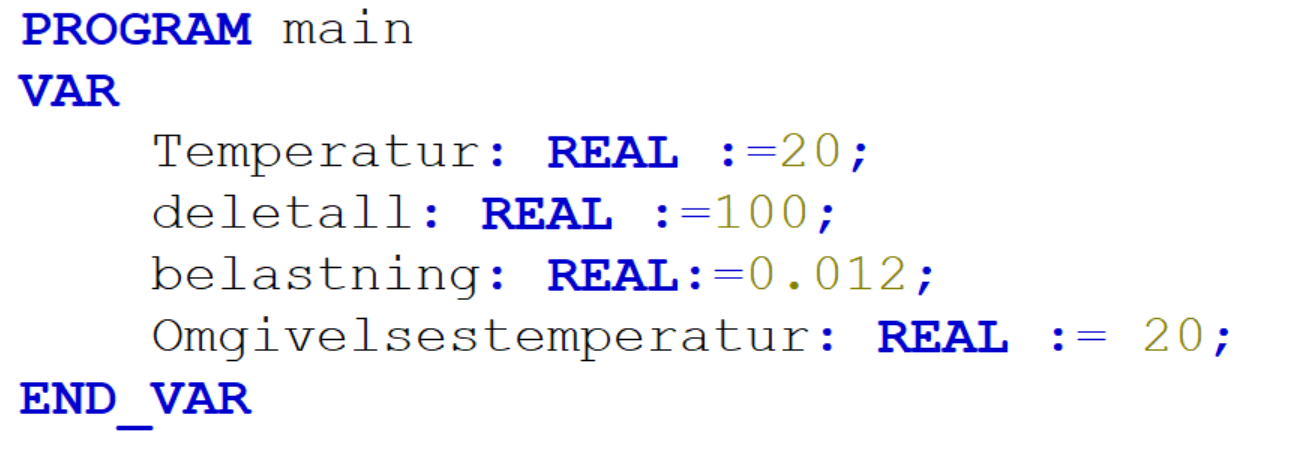
\includegraphics[width=15.5cm]{./aReg2324x05}$$
$$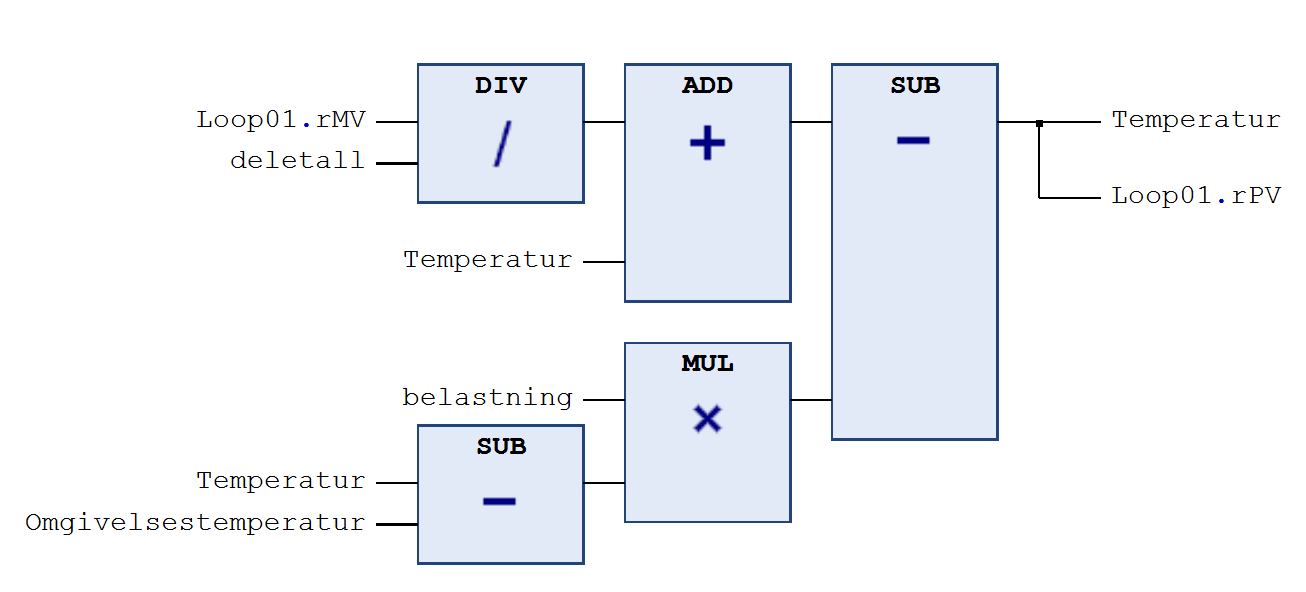
\includegraphics[width=15.5cm]{./aReg2324x06}$$

\textbf{b)}
Utvid programmet med en PID regulator som kan regulere simuleringsmodellen
\vskip 1cm 
\textbf{c)}
Programmer to skalleringsfunksjoner for temperaturtransmitter og reguleringsventil som tilkobles h.h.v. Wago 750-455 (AI 0-32760) og 750-555 (AO 0-32767). Disse to nettene skal kommenteres ut slik at de ikke er aktive i programmet. 
\vskip 1cm 

\vfil \eject
\oppgave{}%8
% Elektroteknikk
\textbf{a)}\\
\vskip 1cm 
Du skal lagen HMI styring til reguleringen av den simulerte modellen av et temperaturreguleringssystem. Det skal bestå av tre bilder:
\begin{itemize}
	\item Hovedmeny
	\item L3 P \& ID "bilde" av prosessen
	\item L4 Optimaliseringsbilde av prosessen
\end{itemize}

På L3 bildet skal det byttes faceplate når en hoder musen over ventilen. 


$$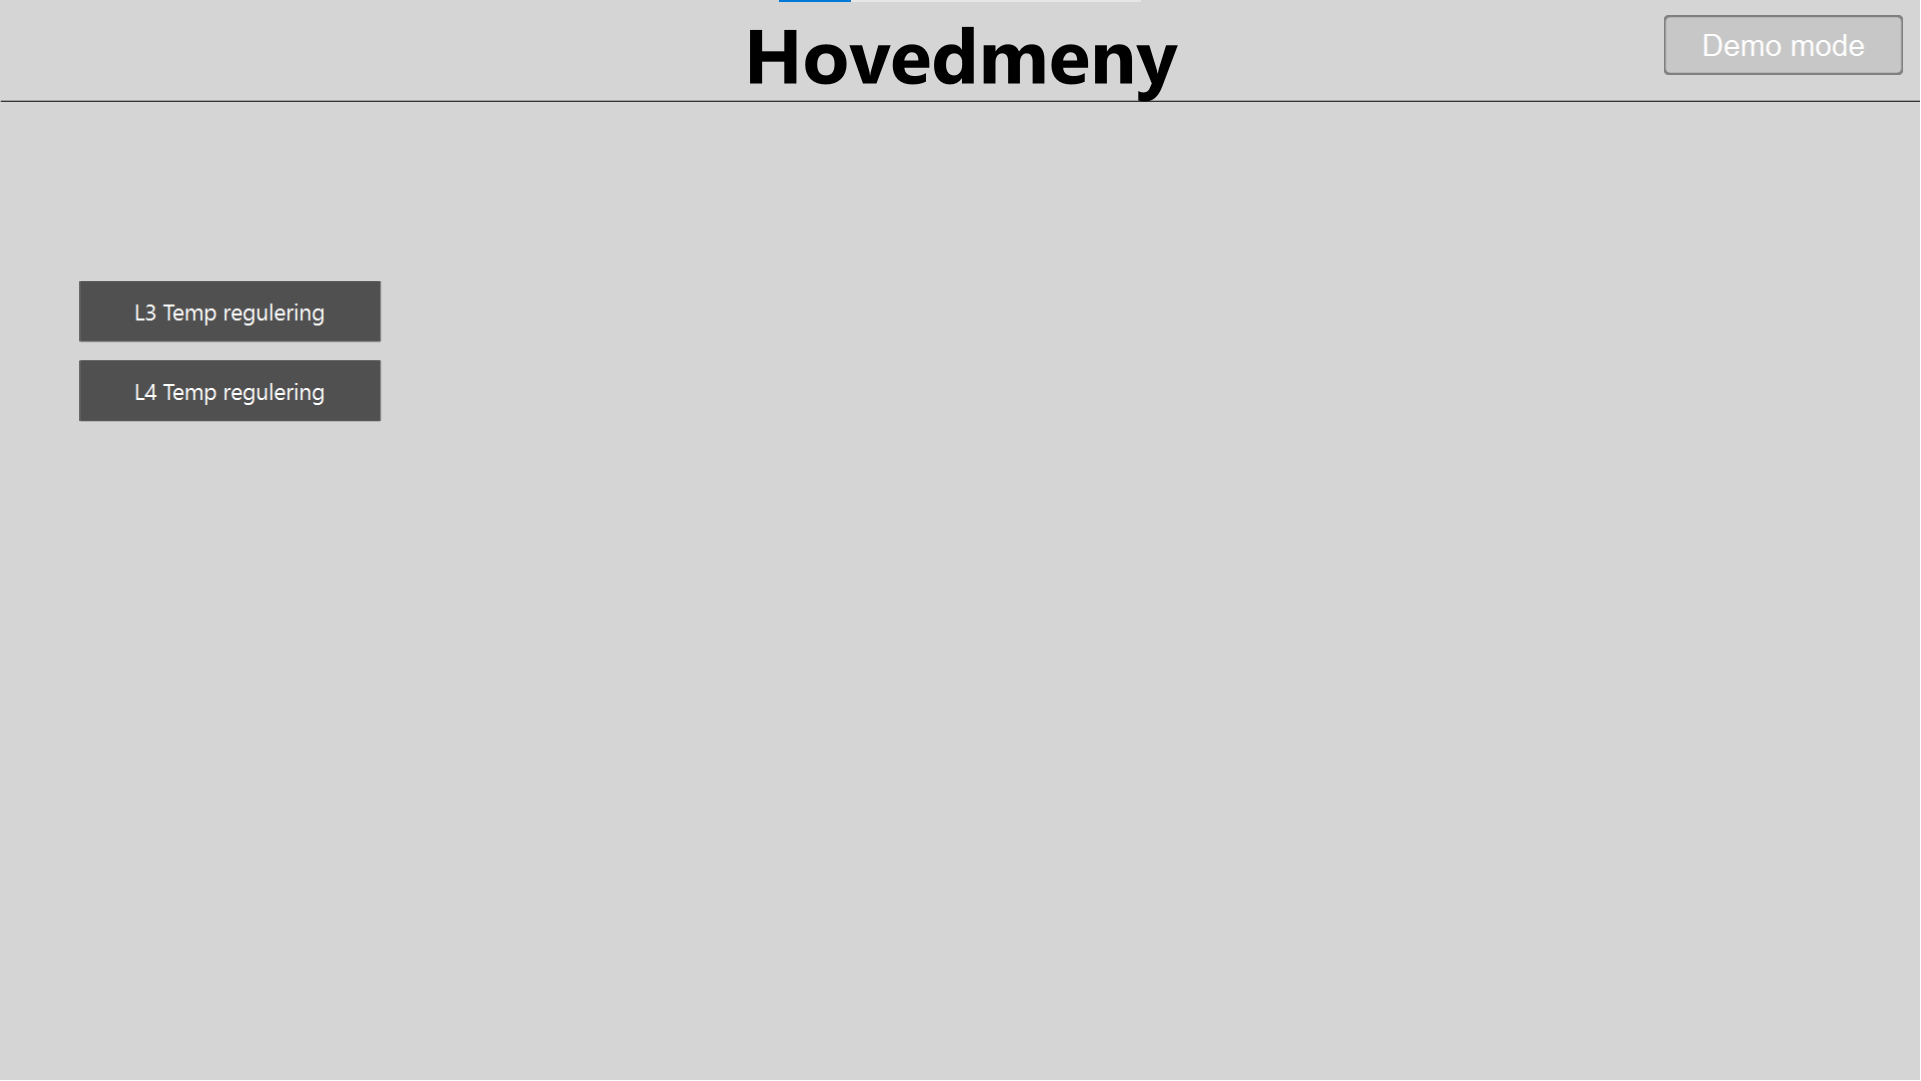
\includegraphics[width=15.5cm]{./aReg2324x03}$$
$$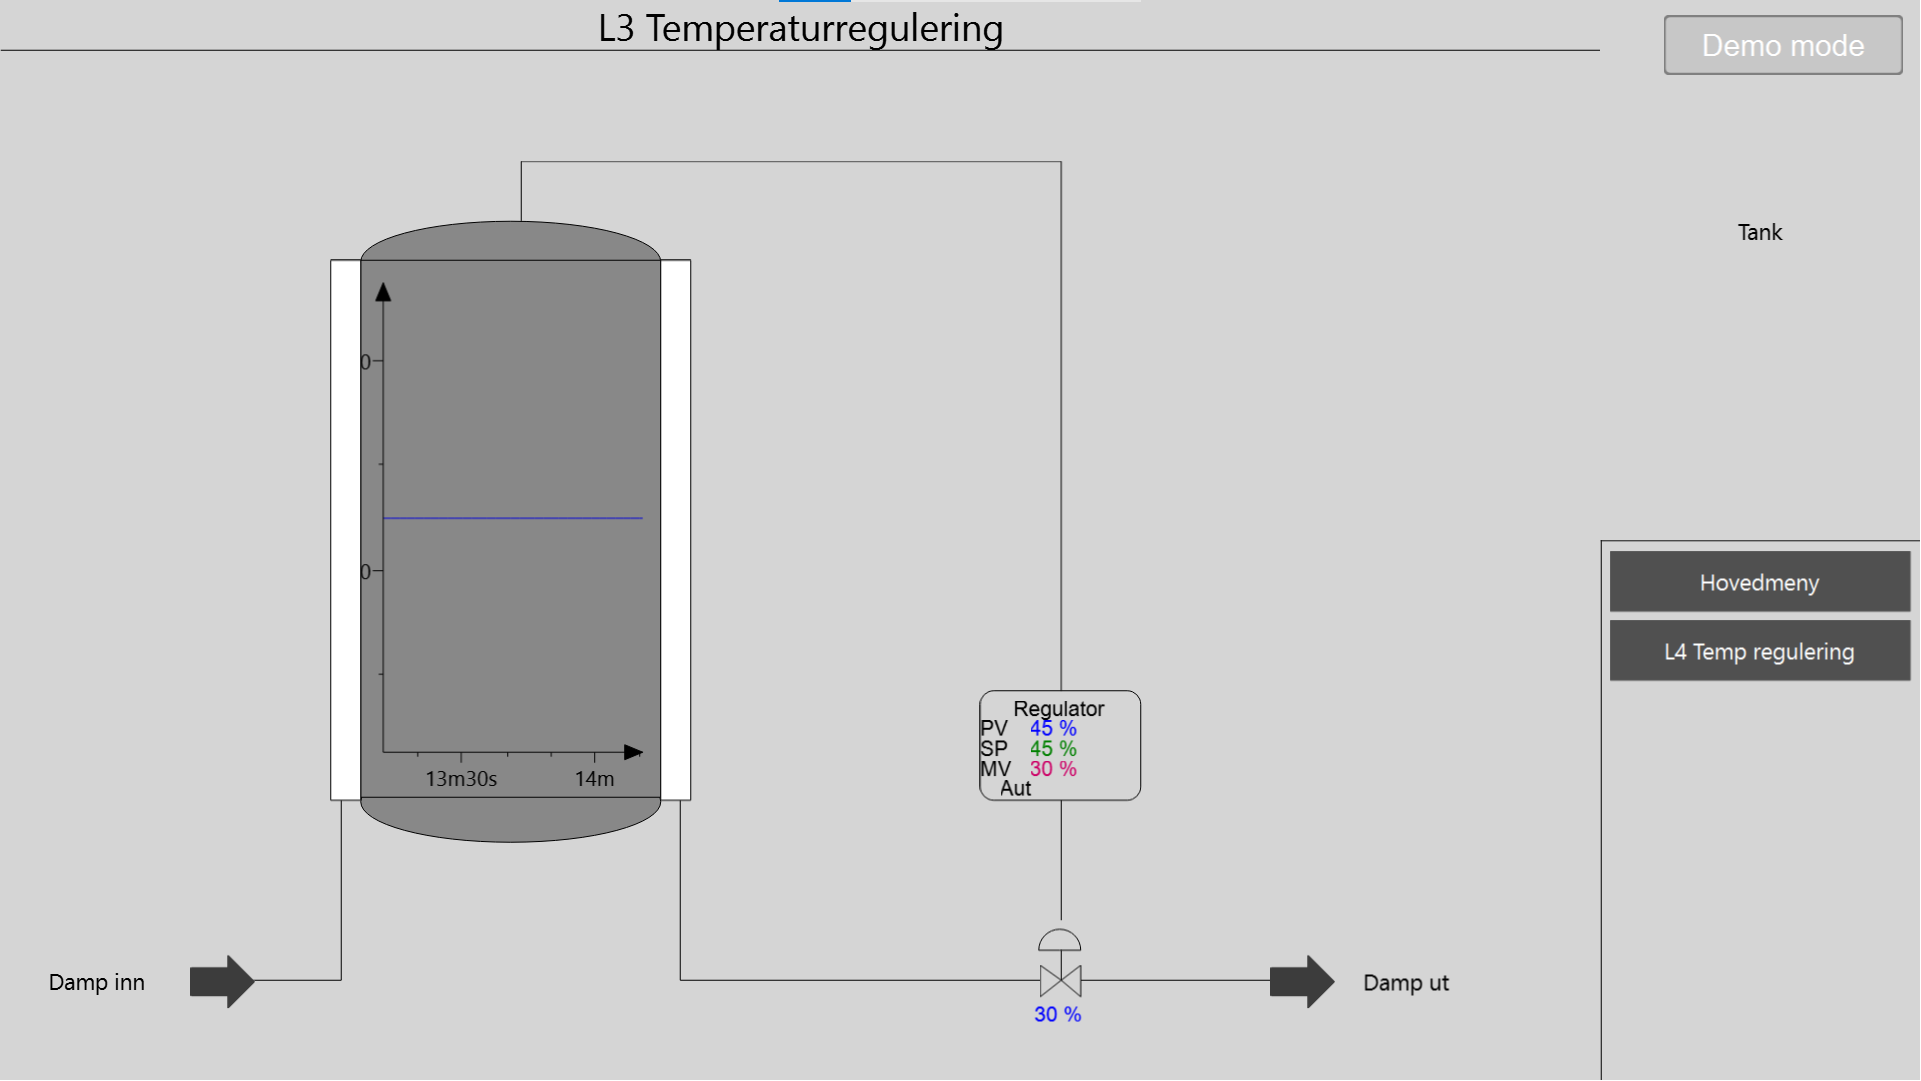
\includegraphics[width=15.5cm]{./aReg2324x02}$$
$$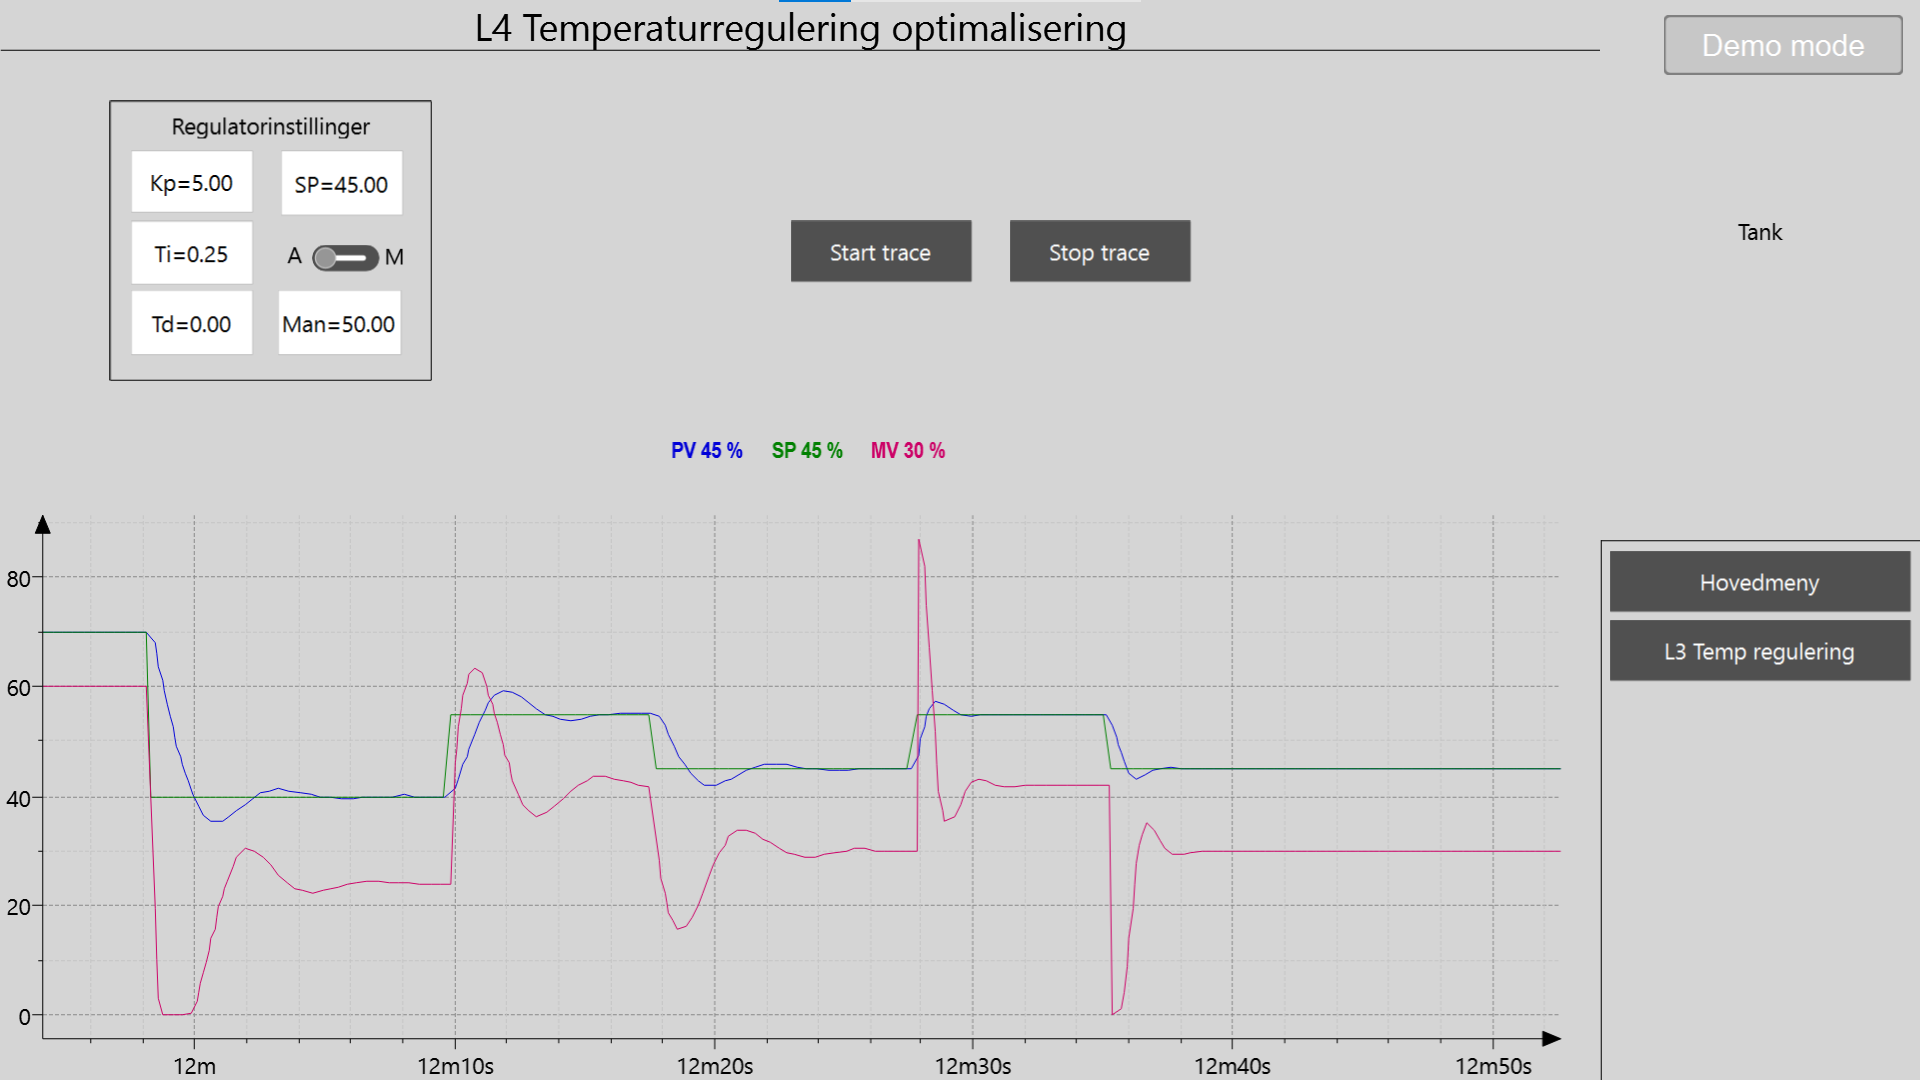
\includegraphics[width=15.5cm]{./aReg2324x01}$$

\vfil \eject
\oppgave{}%9
% Elektroteknikk
\textbf{a)}\\
Du har fått i oppdrag i å montere og koble opp (ikke programmere) et Wago TP600 (delenummer 762-5306/8000-0002, size 10") touchpanel. i\\
Vis hvordan du ville planlagt, gjennomført og dokumentert oppdraget.
\vskip 2 cm 
Dokumentasjon på panelet sende til den epost når prøven starter. 
\vskip 1cm 


\begin{tikzpicture}
	\draw[step=0.5cm,gray!20,very thin]  grid (16,2) ;
\end{tikzpicture}

\textbf{b)}
Oppgavetekst
\vskip 1cm 

\begin{tikzpicture}
	\draw[step=0.5cm,gray!20,very thin]  grid (16,2) ;
\end{tikzpicture}

\vfil \eject
\includepdf[pages=-,angle=90]{../eq/afgvformler.pdf}
\end {document}
